%% Example data sheet
%% Feel free to modify and use this file for any purpose, under
%% either the LaTeX Project Public License or under public domain.

% Options here are passed to the article class.
% Most common options: 10pt, 11pt, 12pt
\documentclass[10pt]{datasheet}

% Input encoding and typographical rules for English language
\usepackage[utf8]{inputenc}
\usepackage[english]{babel}
\usepackage[english]{isodate}

% tikz is used to draw images in this example, but you can
% also use \includegraphics{}.
\usepackage{tikz}
\usepackage{pgfplots}
\usepackage{circuitikz}
\usetikzlibrary{calc}

% These define global texts that are used in headers and titles.
\title{Móra Space Module\hfill
\includegraphics[width=0.09\textwidth]{szte}\hspace{0.3cm}
\includegraphics[width=0.09\textwidth]{mora}}

\date{October 2022}
\revision{Revision 1}



\begin{document}
\maketitle

\section{Features}

\begin{itemize}
	\item{- 40 to 85 \textdegree C temperature range \\ (Guaranteed by design but not characteristic.)}
\item{Redundant oscillator circuit}
\item{Based on Stm32L010F4P6}
\item{Temperature stable passive components}
\item{Ultra wide range power supply : 2.7 - 4.5 V}
\end{itemize}

\section{Applications}

\begin{itemize}
\item{Hall effect measurement}
\item{Temperature measurement}
\item{ADC noise measurement}
\item{Quotes sending}
\end{itemize}

\section{General Description}
This year, on the last day of September, a unique offer was given for the students to create their payload for the MRC-100 satellite. We have accepted the opportunity with great pleasure. Immediately we began brainstorming about the experiments the card should do with the participation of Physics and Engineering students. Finally, the primary experiment was designed to be a noise measurement of the ADC controller. The question is if the noise on the AD samples in the used STM microcontroller is dependent on the radiance of space. Measures will be done at different parts of the trajectory.
The secondary experiment is the jitter measurement of the other modules. The common bus will let us listen and measure the bit rate of the other modules. As a result, we expect to see whether the timing is as important and sensitive point of the design as we see it now.
Our third experiment is about our local culture. In this mode of operation, the satellite will transmit our local student sayings and quotes to show the diversity of our community. 
Our fourth experiment simply measures the magnetic field through the PCB.


% Switch to next column
\vfill\break

\begin{figure}[h]
    \begin{circuitikz}[european]
        \node[op amp] (amp1) {};
        \node[op amp, below = 0.5cm, xscale = -1] (amp2) {};
        \draw (amp1.out) |- (amp2.-);
        \draw (amp2.-) ++(0, 0.3cm) node[circ]{} to +(2,0) node[above left]{5};
        \draw (amp2.out) to (amp1.+);
        \draw (amp1.+) ++(0, -0.3cm) node[circ]{} to +(-2,0) node[above right]{2};
        \draw (amp1.-) to +(-2,0) node[above right]{1};
        \draw (amp2.+) to +(2,0) node[above left]{4};
        \draw (amp1.out) +(0,0.5cm) node (Vdd) {$\mathrm{V_{DD}}$};
        \draw (Vdd.east) to +(1.5,0) node [above left]{6};
        \draw (amp2.out) +(0,-0.5cm) node (Vss) {$\mathrm{V_{SS}}$};
        \draw (Vss.west) to +(-1.6,0) node [above right]{3};
        \draw ($(amp1.north west) + (-0.5,0.5)$) rectangle ($(amp2.south west) + (0.5,-0.5)$);
    \end{circuitikz}
    \caption{Pinout and internal circuit}
\end{figure}

\begin{figure}[h]
    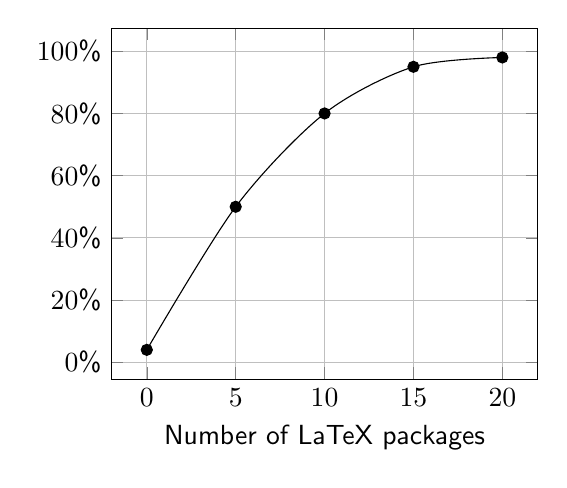
\begin{tikzpicture}
        \sffamily
        \begin{axis}[
            width=7cm,
            xlabel={Number of LaTeX packages},
            ytick distance=20,
            yticklabel={\pgfmathprintnumber{\tick}\%},
            xmajorgrids, ymajorgrids]
        \addplot[smooth,mark=*] plot coordinates {
            (0,4)
            (5,50)
            (10,80)
            (15,95)
            (20,98)
        };
        \end{axis}
    \end{tikzpicture}
    \caption{Typical data sheet production efficiency}
\end{figure}

% For wide tables, a single column layout is better. It can be switched
% page-by-page.
\onecolumn


\section{Electrical Specifications}
All specifications are in $-40\degree C \leq T_A \leq 85\degree C$ unless otherwise noted.

\begin{table}[h]
\begin{threeparttable}
	\caption{Electrical characteristic specifications}
\begin{tabularx}{\textwidth}{l | c | c c c | c | X}
    \thickhline
    \textbf{Parameter} & \textbf{Symbol} & \textbf{Min.} & \textbf{Typ.} & \textbf{Max.} &
    \textbf{Unit} \\
    \hline
    Current consumption  & $I_S$ & 10 & 10 & 10 & mA  \\
	Standby current consumption & $I_B$ & 10 & 10 & 10 & mA \\
	Additional current consumption with Oscillator On & $I_O$ & 10 & 10 & 10 & mA \\
	Additional current consumption with Hall sensor On & $I_H$ & 10 & 10 & 10 & mA \\
	Additional current consumption with Temperature sensor On & $I_T$ & 10 & 10 & 10 & mA \\
    \thickhline
\end{tabularx}
\begin{tablenotes}
\item[1]{Based on characterization data, not tested in production.}
\end{tablenotes}
\end{threeparttable}
\end{table}



\section{Dimensions}

\begin{table}[h]
\caption{Board Dimensions}
\begin{tabularx}{\textwidth}{l | X}
    \thickhline
    \textbf{Parameter} & \textbf{Size} \hspace{5cm} \\
    \hline
    Side & 30.0 x 30.0  \\
	Height & 3.0 \\
    \thickhline
\end{tabularx}
	\begin{tablenotes}
	\item[1]{Dimensions are expressed in millimeters.}
	\end{tablenotes}
\end{table}





\textbf{Note:} Stresses above those listed under Absolute Maximum Ratings can
cause permanent damage to the device. This is a stress rating only. Functional
operation of the device is not implied in any conditions above those indicated
in the Electrical Specifications section.

\begin{figure}
	\centering
	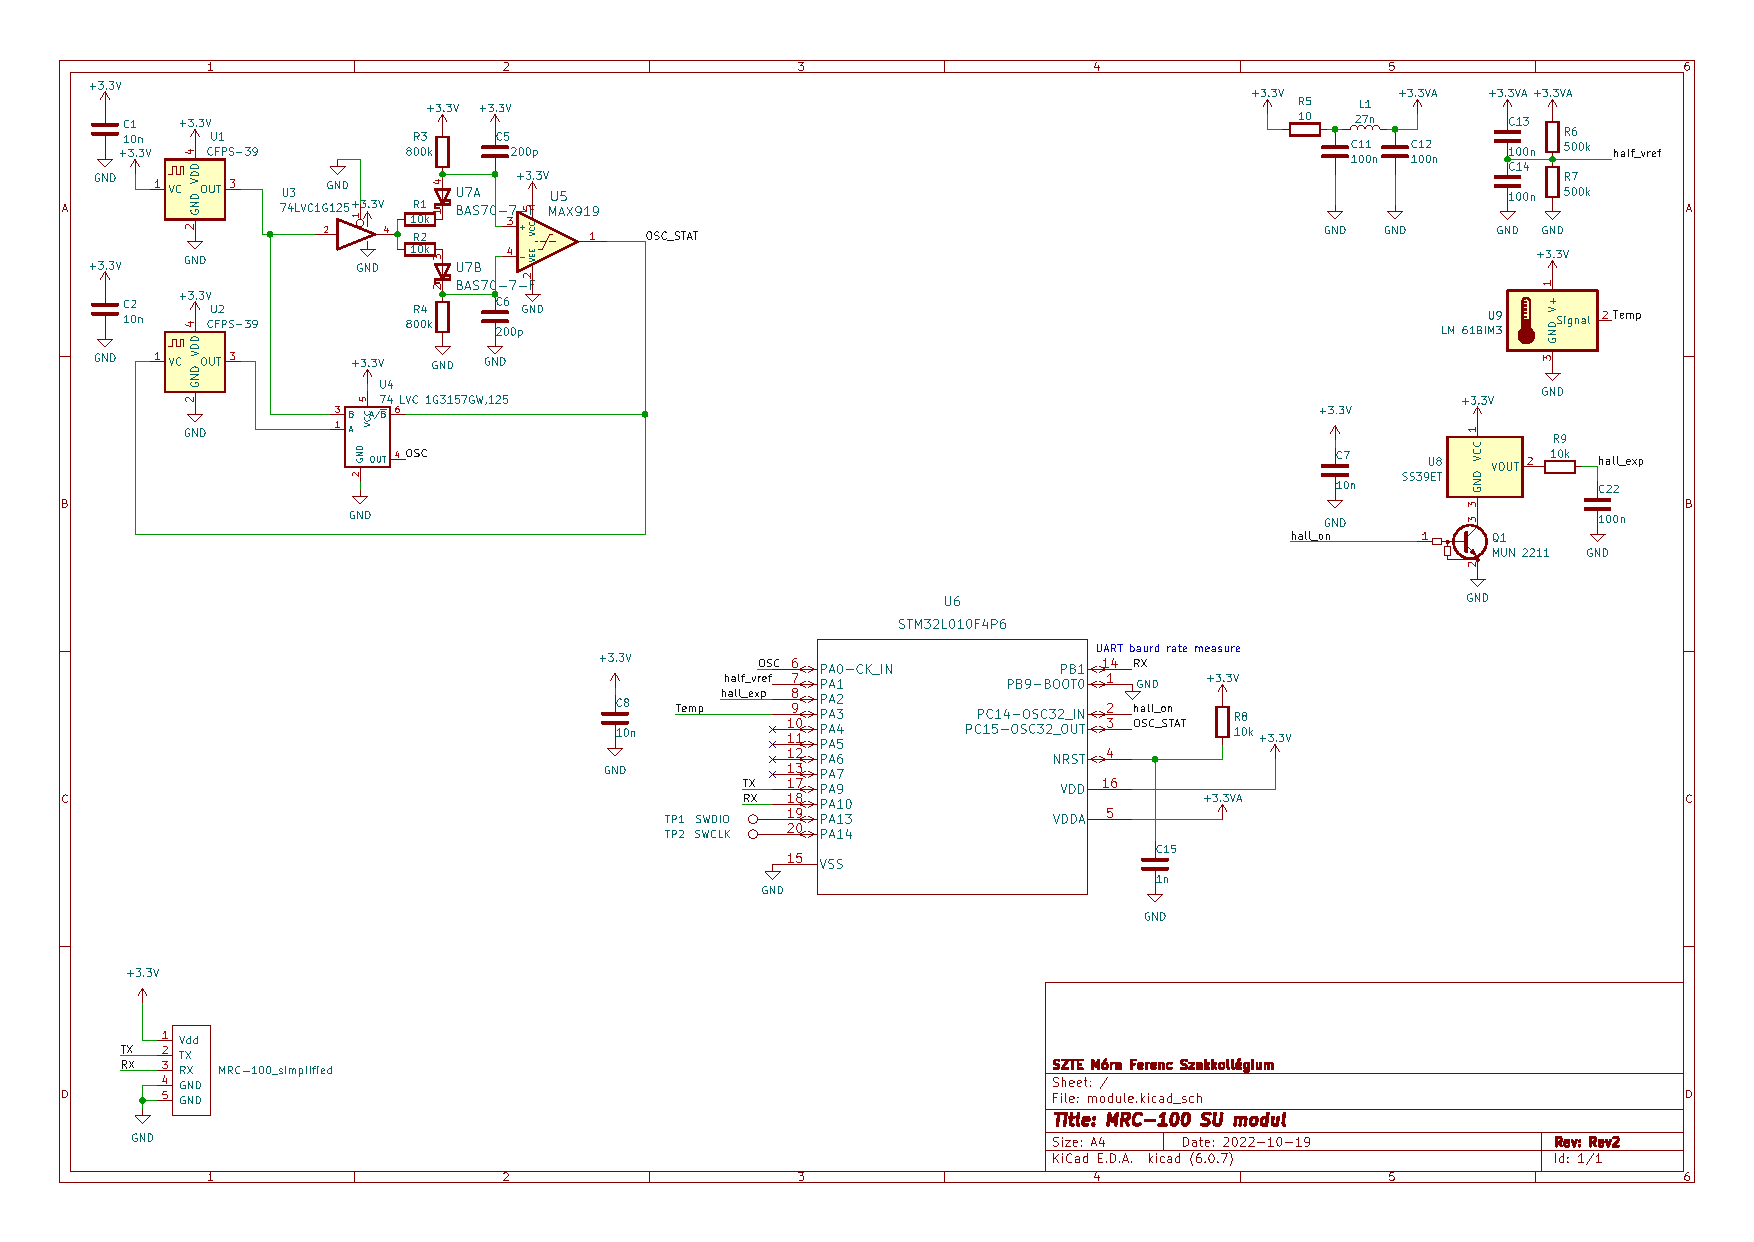
\includegraphics[width=1.2\textwidth,angle = 90]{sch}
	\caption{Schematics}
\end{figure}

\end{document}



